\documentclass[11pt]{article}

\usepackage[margin=1in]{geometry}
\usepackage{graphicx}
\usepackage{booktabs}
\usepackage{amsmath}
\usepackage{siunitx}
\usepackage[hidelinks]{hyperref}

% Figures live with the run they came from, not copied in.
\graphicspath{{../runs/bulgedisk_long/}}

\newcommand{\arcsec}{\ensuremath{^{\prime\prime}}}
\newcommand{\thetaE}{\ensuremath{\theta_{\mathrm{E}}}}
\newcommand{\chisqv}{\ensuremath{\chi^{2}_{\nu}}}

\title{A bulge$+$disk lens model for DESI238}
\author{Claude\thanks{Claude Code (Anthropic). An AI wrote the modelling pipeline in
\texttt{claude/pipeline/}, ran the fits, and drafted this report. The pipeline is a
driver for GIGA-Lens (\href{https://github.com/giga-lens/gigalens}{giga-lens/gigalens}),
which does the rendering and inference; the vendored package was not modified. The HST
observations, the choice of target, and the direction of the analysis at every branch
point came from the repository owner. Every number traces to
\texttt{runs/bulgedisk\_long/} and to \texttt{RESULTS\_v3.md}; the tables were transcribed
from \texttt{params.csv} by hand and have not been checked programmatically against it.}}
\date{31 July 2026}

\begin{document}
\maketitle

\begin{abstract}
We model the strong lens DESI238 (HST WFC3/IR, F140W, $80\times80$ pixels at
$0.065\arcsec$) with GIGA-Lens' MAP$\rightarrow$SVI$\rightarrow$HMC sequence. The adopted
model has an EPL$+$external-shear deflector, a two-component (bulge$+$disk) deflector
light profile, and a two-component S\'ersic source: 36 free parameters. It gives
$\chisqv = 0.989$ and is preferred over the single-component deflector light by
$\Delta\mathrm{BIC} \approx -1762$. The Einstein radius is
$\thetaE = 1.480 \pm 0.003\arcsec$ (\mbox{$\hat{R} = 1.001$}, $\mathrm{ESS} = 94{,}186$).
A single-source, single-lens-light fit of the same data gave $1.516 \pm 0.002\arcsec$, but
that model is rejected by the data at $\Delta\mathrm{BIC} \approx -5294$ and is superseded
rather than competing; the $0.036\arcsec$ difference is therefore a bias removed, not a
systematic uncertainty to be carried.
\end{abstract}

\section{Data and model}

The cutout is $80\times80$ pixels at $0.065\arcsec\,\mathrm{pix}^{-1}$, extracted from the
\texttt{final\_94\_drz.fits} drizzle product in units of $\mathrm{e^{-}\,s^{-1}}$, with
$t_{\mathrm{exp}} = 1197.699\,\mathrm{s}$. The PSF is a $27\times27$ kernel at the same
pixel scale, normalised to unit sum. Rendering uses $2\times$ supersampling.

The noise model is the GIGA-Lens \texttt{ForwardProbModel}, whose per-pixel dispersion
%
\begin{equation}
  \sigma = \sqrt{\sigma_{\mathrm{bkg}}^{2} + \max(m,0)/t_{\mathrm{exp}}}
\end{equation}
%
depends on the model image $m$ and so is re-evaluated every step. We take
$\sigma_{\mathrm{bkg}} = 0.0075\,\mathrm{e^{-}\,s^{-1}}$, the median of six widely
separated blank patches in the parent frame; the patch-to-patch range is
$0.0070$--$0.0092$, and \S\ref{sec:noise} shows what that range does to \chisqv.

The model has three blocks:

\begin{itemize}
  \item \textbf{Mass}: an elliptical power law (EPL) plus external shear, eight
    parameters.
  \item \textbf{Deflector light}: two S\'ersic profiles, given \emph{different} priors
    because a bulge and a disk are physically distinct and identical priors would add a
    label-switching mode for nothing.
  \item \textbf{Source light}: two S\'ersic profiles with the same (wide) prior.
\end{itemize}

Inference is 1024-start Adam (350 steps), then a full-covariance Gaussian SVI ansatz
(1500 steps, warmup-then-decay schedule peaking at $2\times10^{-3}$), then 50 chains of
preconditioned HMC, 3000 draws after 1000 burn-in. Everything internal is in unconstrained
space; the tables below are after applying the prior's bijector.

\section{The fit}

\begin{figure}[htbp]
  \centering
  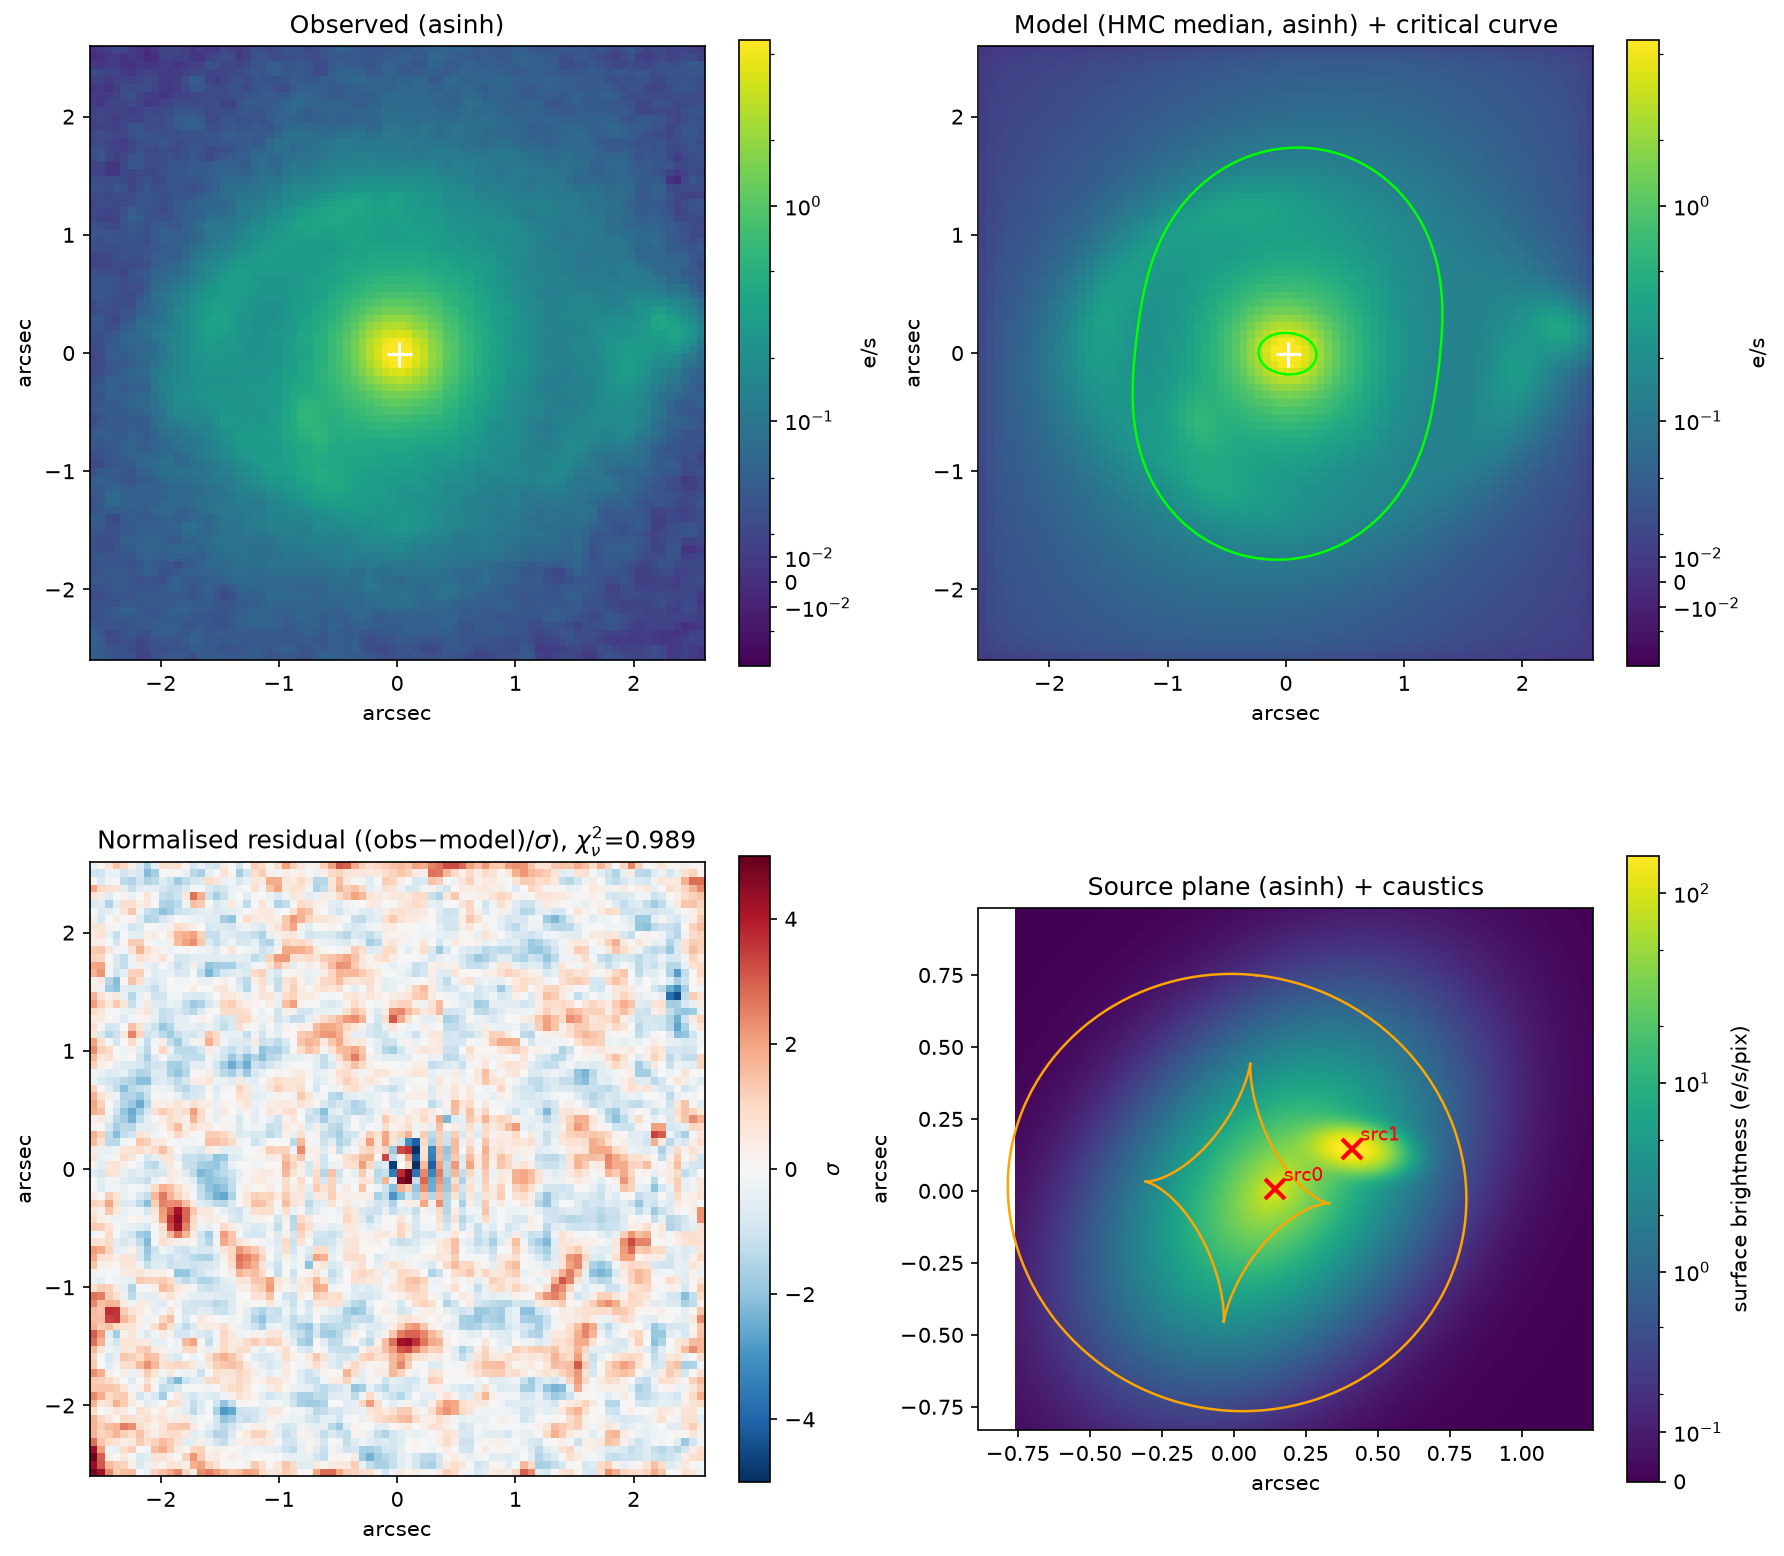
\includegraphics[width=\textwidth]{lensing_overview.png}
  \caption{Observed image, model, normalised residual, and reconstructed source plane.
    The first, second, and fourth panels use an \texttt{asinh} stretch; the observed and
    model panels share a single normalisation so they are directly comparable by eye. The
    linear width of the stretch is $5\sigma_{\mathrm{bkg}}$, so the linear regime covers
    exactly those pixels consistent with background. Solid curves are the tangential and
    radial critical curves (panel 2) and their caustics (panel 4). The tangential critical
    curve has mean radius $1.545\arcsec$ against $\thetaE = 1.480\arcsec$, a $4.4\%$
    difference --- the expected offset for an elliptical, non-isothermal
    ($\gamma = 1.79$) deflector, and a check that the Jacobian orientation is right.}
  \label{fig:overview}
\end{figure}

The residual panel of Figure~\ref{fig:overview} is featureless at the level of the arcs.
Two things in it are worth flagging rather than passing over:

\begin{itemize}
  \item A one-pixel-period vertical striping survives in the core at $\pm5\sigma$. An
    earlier round attributed this to a saturating diverging colormap on a smooth dipole,
    but that argument was checked against the \emph{model}, not this residual, and a
    one-pixel period is not what a colormap artifact on a smooth field looks like. It is
    unresolved.
  \item The \texttt{lens\_light1} disk has $R_{\mathrm{sersic}} = 2.59\arcsec$, larger
    than the $2.6\arcsec$ half-width of the cutout. It is extrapolating over most of its
    own scale length, and should be re-checked against a larger crop before its
    parameters are read physically.
\end{itemize}

\section{Parameters}

All values are posterior medians with $\pm$ the standard deviation, from
$3000 \times 50 = 150{,}000$ draws. Positions are in arcseconds relative to the cutout
centre; $I_{e}$ is in $\mathrm{e^{-}\,s^{-1}\,pix^{-1}}$ at the half-light radius. $\hat{R}$
is the Gelman--Rubin statistic across the 50 chains, and ESS the bulk effective sample
size.

\begin{table}[htbp]
  \centering
  \caption{Mass model: elliptical power law plus external shear. Every parameter has
    $\hat{R} \le 1.002$; the non-convergence discussed in \S\ref{sec:conv} does not touch
    this block.}
  \label{tab:mass}
  \begin{tabular}{llS[table-format=-1.6]S[table-format=1.6]S[table-format=1.3]S[table-format=6.0]}
    \toprule
    Profile & Parameter & {Median} & {$\sigma$} & {$\hat{R}$} & {ESS} \\
    \midrule
    EPL   & $\thetaE$ (\arcsec)  &  1.479641 & 0.002826 & 1.001 & 94186 \\
          & $\gamma$             &  1.792080 & 0.021054 & 1.000 & 61723 \\
          & $e_{1}$              &  0.023899 & 0.006020 & 1.002 & 95960 \\
          & $e_{2}$              &  0.016562 & 0.005270 & 1.001 & 89243 \\
          & $x_{0}$ (\arcsec)    &  0.013761 & 0.002966 & 1.001 & 48625 \\
          & $y_{0}$ (\arcsec)    & -0.005085 & 0.003031 & 1.001 & 44694 \\
    \midrule
    Shear & $\gamma_{1}$         &  0.142112 & 0.004309 & 1.001 & 91224 \\
          & $\gamma_{2}$         & -0.015412 & 0.003681 & 1.001 & 86078 \\
    \bottomrule
  \end{tabular}
\end{table}

Two features of Table~\ref{tab:mass} deserve comment. First, the external shear is large:
$|\gamma_{\mathrm{ext}} = 0.143|$, some $33\sigma$ from zero, which is well above what a
typical field produces and should be checked against the galaxies visible in the parent
drizzle frame. Second, the mass parameters are strongly correlated
(Figure~\ref{fig:corner_mass}); in particular $\gamma_{2}$ and $e_{2}$ have
$r = +0.947$, so the marginals $e_{2} = 0.017 \pm 0.005$ and
$\gamma_{2} = -0.015 \pm 0.004$ are emphatically not two independent measurements. This is
the familiar ellipticity--shear degeneracy of EPL$+$shear, and it is the reason to quote
\thetaE, which is nearly orthogonal to it, rather than the shape parameters.

\begin{table}[htbp]
  \centering
  \caption{Light profiles. The deflector's two components separate cleanly into a compact
    bulge and an extended disk, an $8.2\times$ ratio in scale radius from priors that
    overlap at ${\sim}1\sigma$. Rows in the source block marked $\dagger$ are discussed in
    \S\ref{sec:conv}.}
  \label{tab:light}
  \begin{tabular}{llS[table-format=-3.6]S[table-format=2.6]S[table-format=1.3]S[table-format=6.0]}
    \toprule
    Component & Parameter & {Median} & {$\sigma$} & {$\hat{R}$} & {ESS} \\
    \midrule
    \multicolumn{6}{l}{\emph{Deflector light}} \\
    bulge & $I_{e}$                       & 265.609558 & 21.464956 & 1.012 &  3924 \\
    (\texttt{lens\_light0})
          & $R_{\mathrm{sersic}}$ (\arcsec)&  0.316435 &  0.018986 & 1.012 &  4367 \\
          & $n_{\mathrm{sersic}}$         &   3.110604 &  0.101452 & 1.014 &  3687 \\
          & $e_{1}$                       &  -0.006533 &  0.003503 & 1.019 &  3004 \\
          & $e_{2}$                       &  -0.054691 &  0.005968 & 1.040 &  1331 \\
          & $x_{0}$ (\arcsec)             &   0.011480 &  0.000660 & 1.001 & 55351 \\
          & $y_{0}$ (\arcsec)             &   0.008185 &  0.000582 & 1.000 & 75225 \\
    \addlinespace
    disk  & $I_{e}$                       &   8.653830 &  0.850306 & 1.031 &  2017 \\
    (\texttt{lens\_light1})
          & $R_{\mathrm{sersic}}$ (\arcsec)&  2.585748 &  0.120492 & 1.042 &  1594 \\
          & $n_{\mathrm{sersic}}$         &   2.091850 &  0.143315 & 1.096 &   602 \\
          & $e_{1}$                       &  -0.083190 &  0.005385 & 1.004 & 10766 \\
          & $e_{2}$                       &   0.145362 &  0.008455 & 1.010 &  4888 \\
          & $x_{0}$ (\arcsec)             &   0.016332 &  0.004579 & 1.000 & 67916 \\
          & $y_{0}$ (\arcsec)             &   0.003584 &  0.004166 & 1.001 & 61822 \\
    \midrule
    \multicolumn{6}{l}{\emph{Source light}} \\
    host  & $I_{e}$                       &  18.429447 &  0.631662 & 1.003 &106124 \\
    (\texttt{source0})
          & $R_{\mathrm{sersic}}$ (\arcsec)&  0.209440 &  0.006663 & 1.003 & 23248 \\
          & $n_{\mathrm{sersic}}$         &   1.086166 &  0.036213 & 1.002 &110851 \\
          & $e_{1}$                       &  -0.034383 &  0.008562 & 1.001 &104260 \\
          & $e_{2}$                       &   0.186871 &  0.007973 & 1.001 &105610 \\
          & $x_{0}$ (\arcsec)             &   0.144529 &  0.003334 & 1.001 & 42646 \\
          & $y_{0}$ (\arcsec)             &   0.005654 &  0.002808 & 1.002 & 24599 \\
    \addlinespace
    knot  & $I_{e}$                       &  86.815727 &  4.459748 & 1.011 &  6745 \\
    (\texttt{source1})
          & $R_{\mathrm{sersic}}$ (\arcsec)&  0.065510 &  0.002623 & 1.002 & 16883 \\
          & $n_{\mathrm{sersic}}^{\dagger}$&  0.521684 &  0.029147 & 1.338 &   201 \\
          & $e_{1}$                       &   0.318078 &  0.023257 & 1.009 &  5965 \\
          & $e_{2}$                       &  -0.083478 &  0.026384 & 1.005 & 10569 \\
          & $x_{0}$ (\arcsec)             &   0.411215 &  0.010253 & 1.001 & 61416 \\
          & $y_{0}$ (\arcsec)             &   0.146367 &  0.005701 & 1.000 & 63237 \\
    \bottomrule
  \end{tabular}
\end{table}

\begin{figure}[htbp]
  \centering
  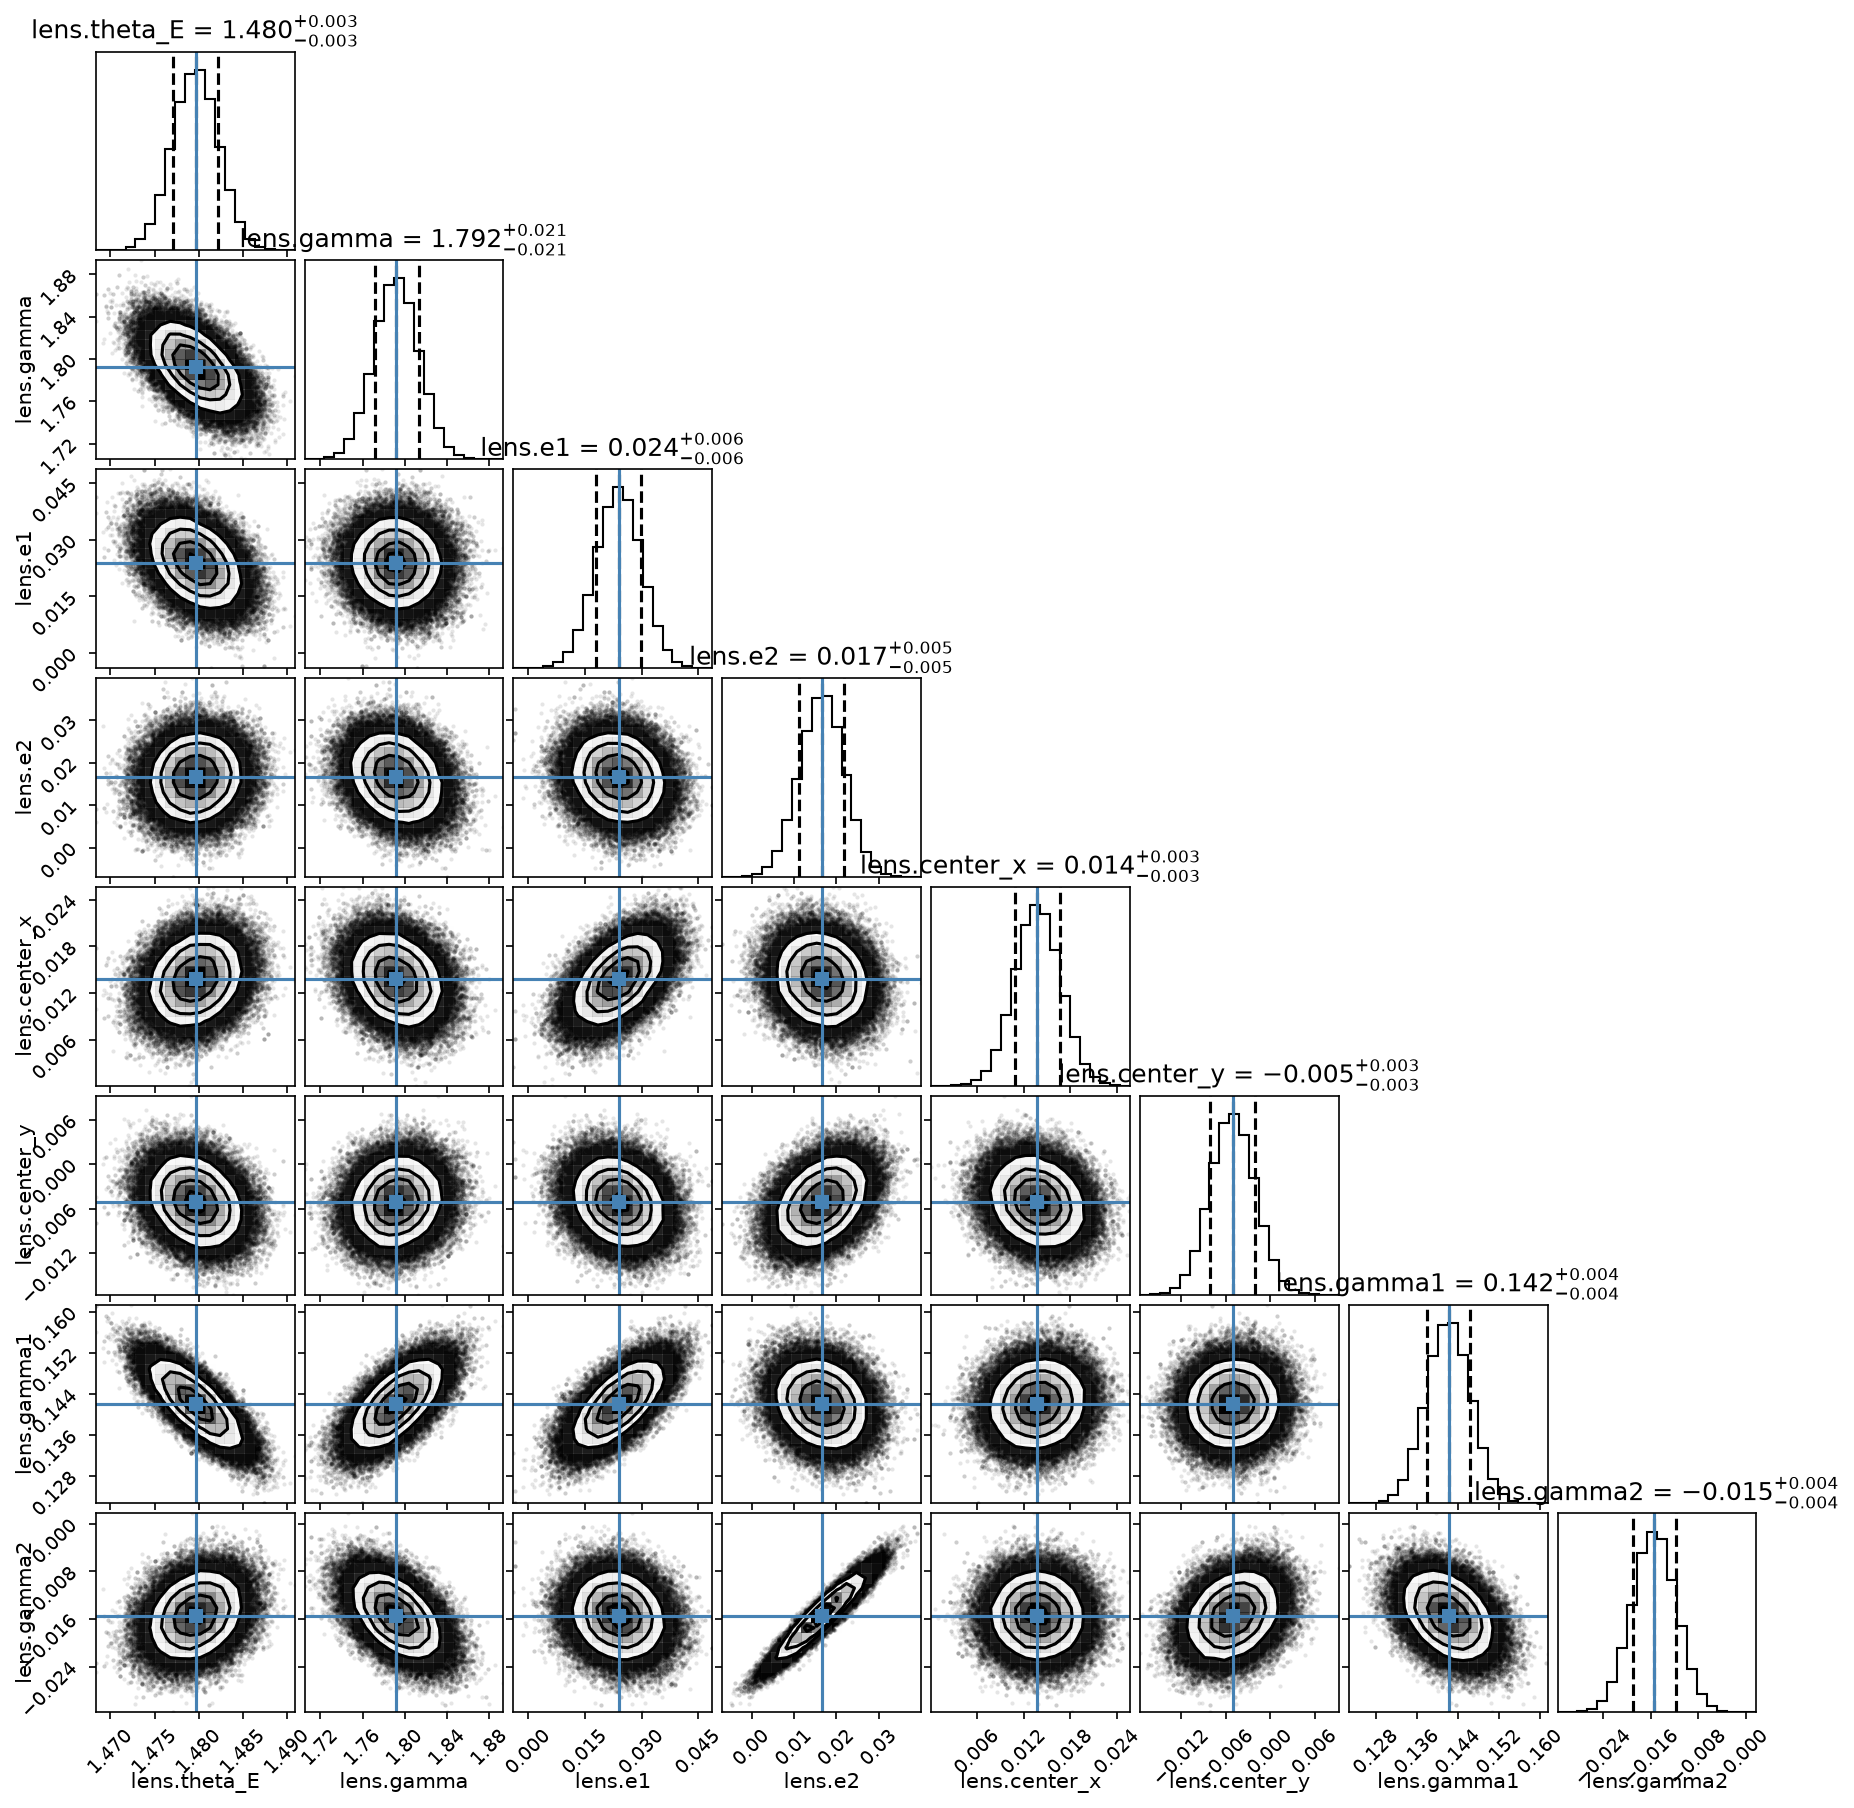
\includegraphics[width=0.85\textwidth]{corner_mass.png}
  \caption{Posterior for the eight mass parameters. The dominant structure is the
    $\gamma_{2}$--$e_{2}$ ridge at $r = +0.947$; $\gamma_{1}$ correlates with \thetaE\ at
    $r = -0.776$ and with $\gamma$ at $r = +0.661$. \thetaE\ itself is the tightest and
    least degenerate direction in the block.}
  \label{fig:corner_mass}
\end{figure}

\begin{figure}[htbp]
  \centering
  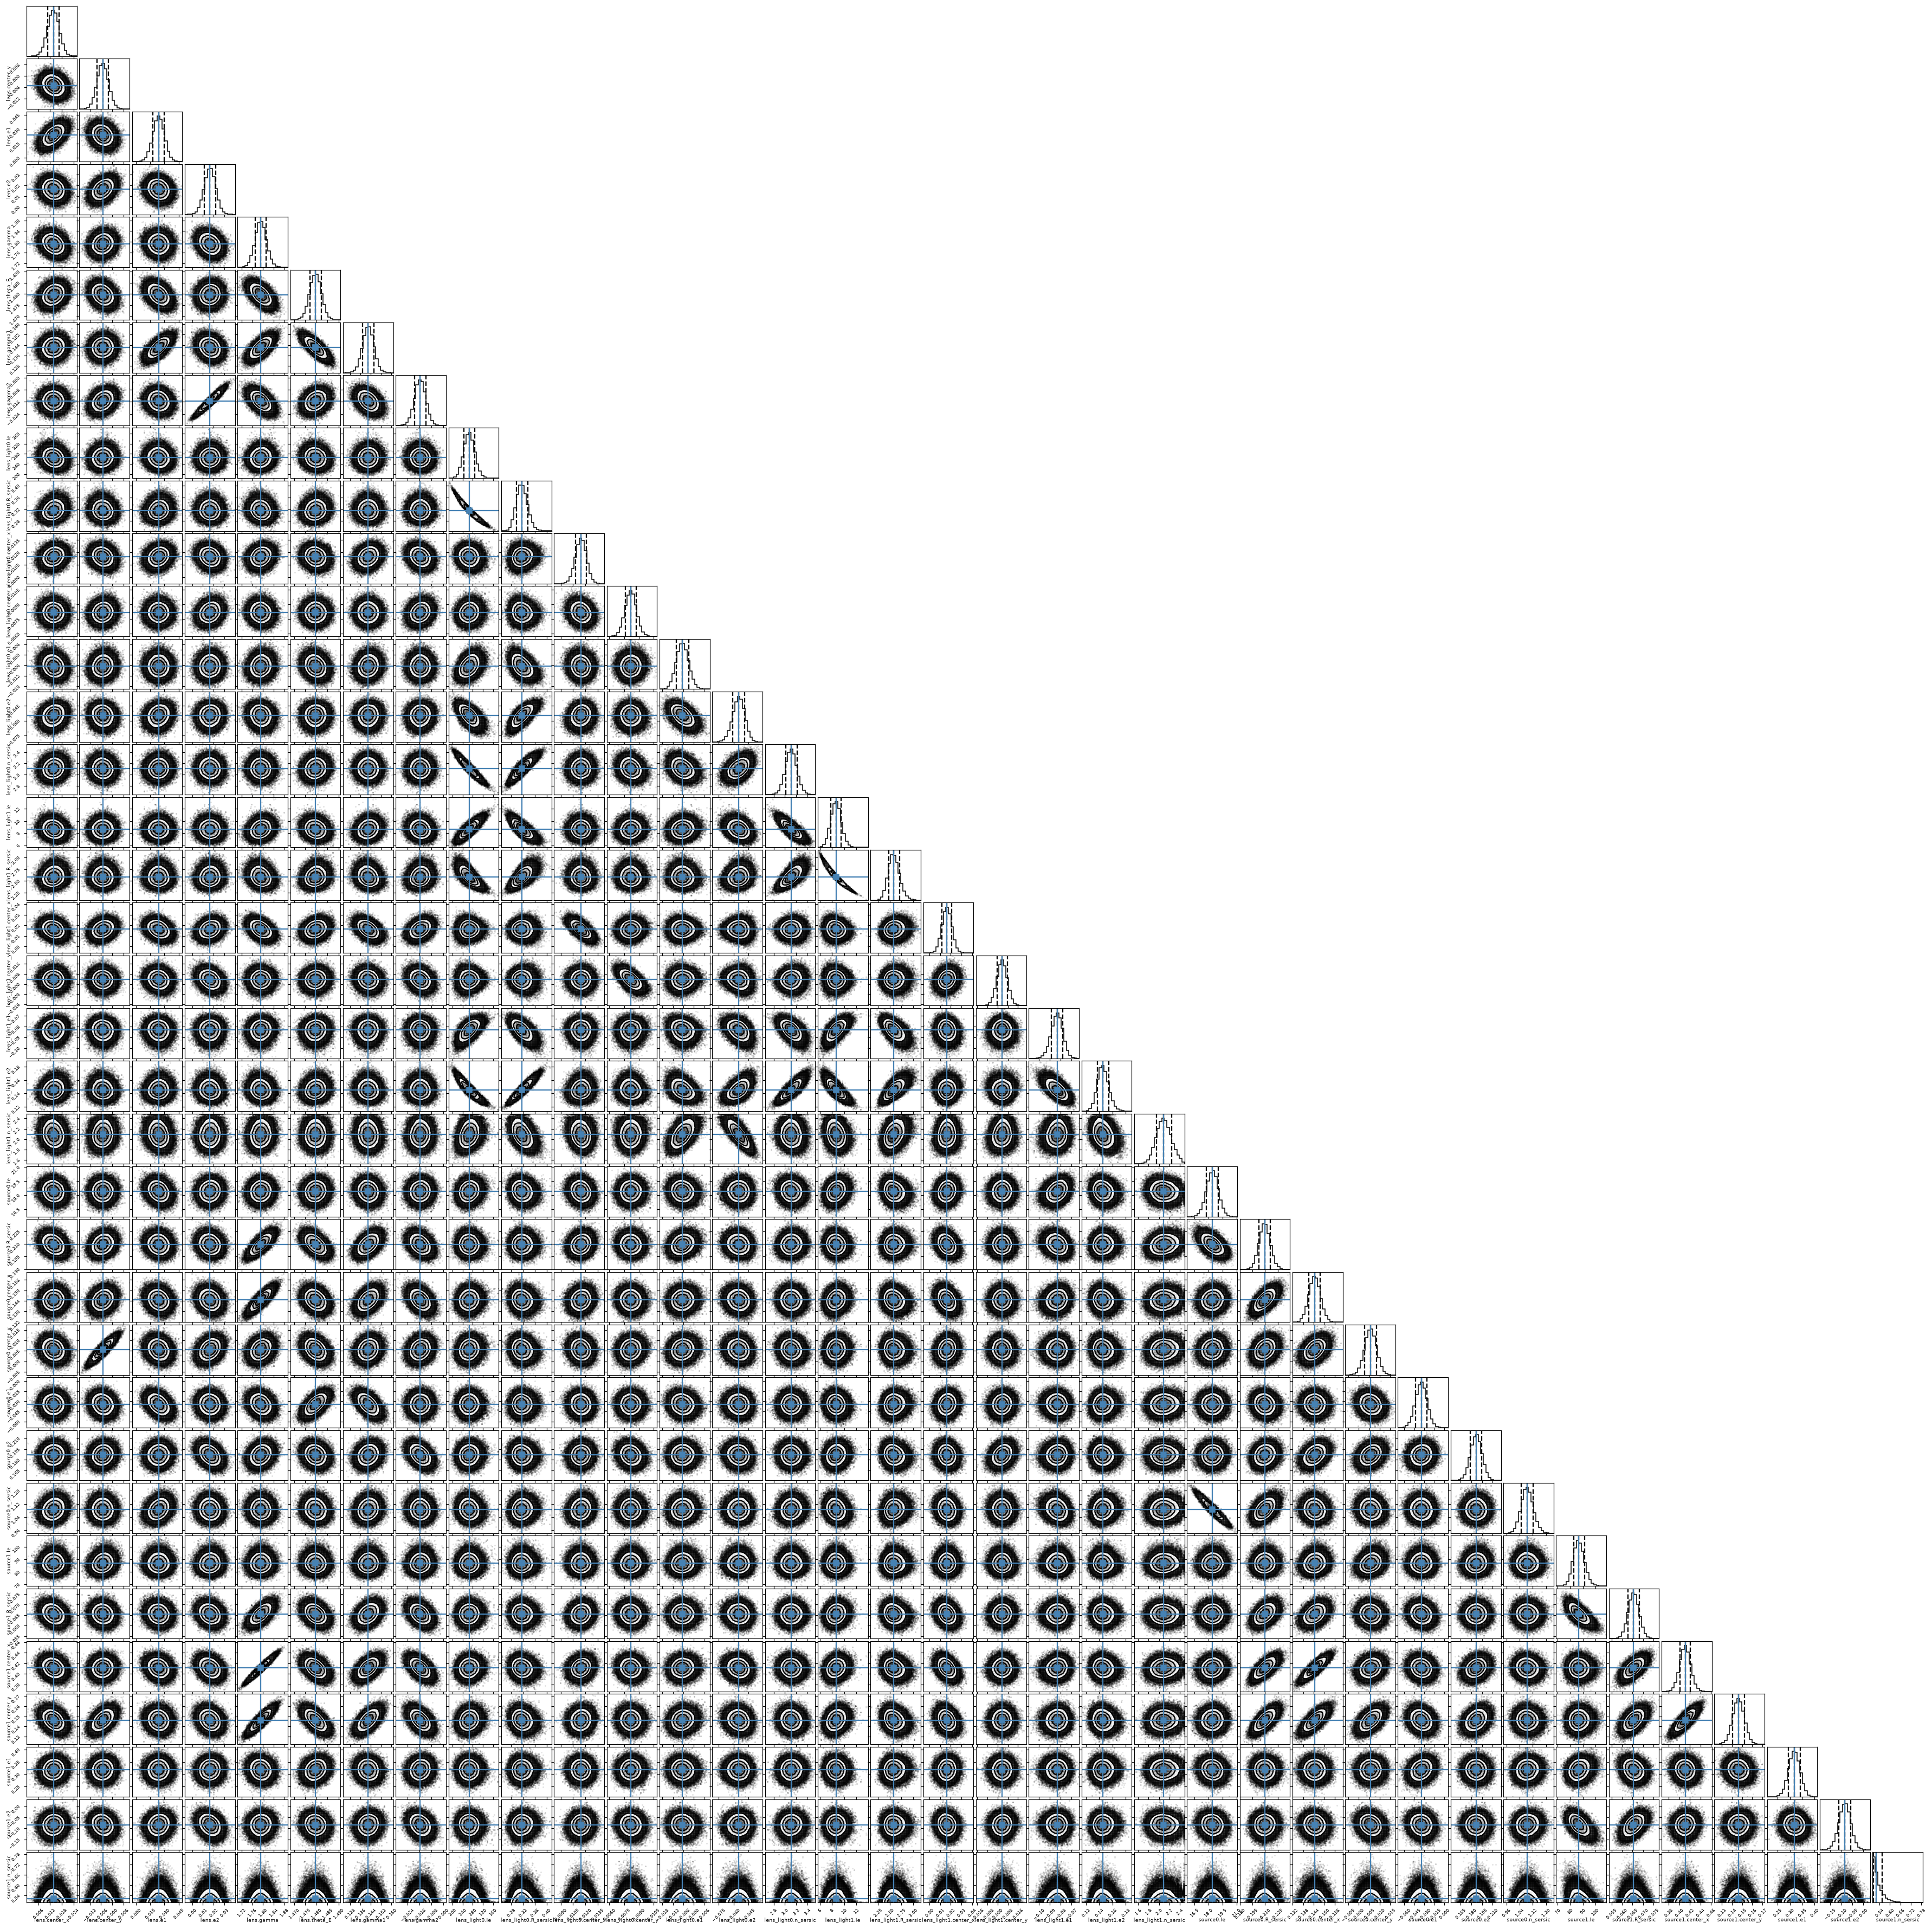
\includegraphics[width=\textwidth]{corner_full.png}
  \caption{Full 36-parameter posterior. Reproduced at reduced size for completeness; the
    machine-readable summary is \texttt{runs/bulgedisk\_long/params.csv}.}
  \label{fig:corner_full}
\end{figure}

\section{The source}

\begin{figure}[htbp]
  \centering
  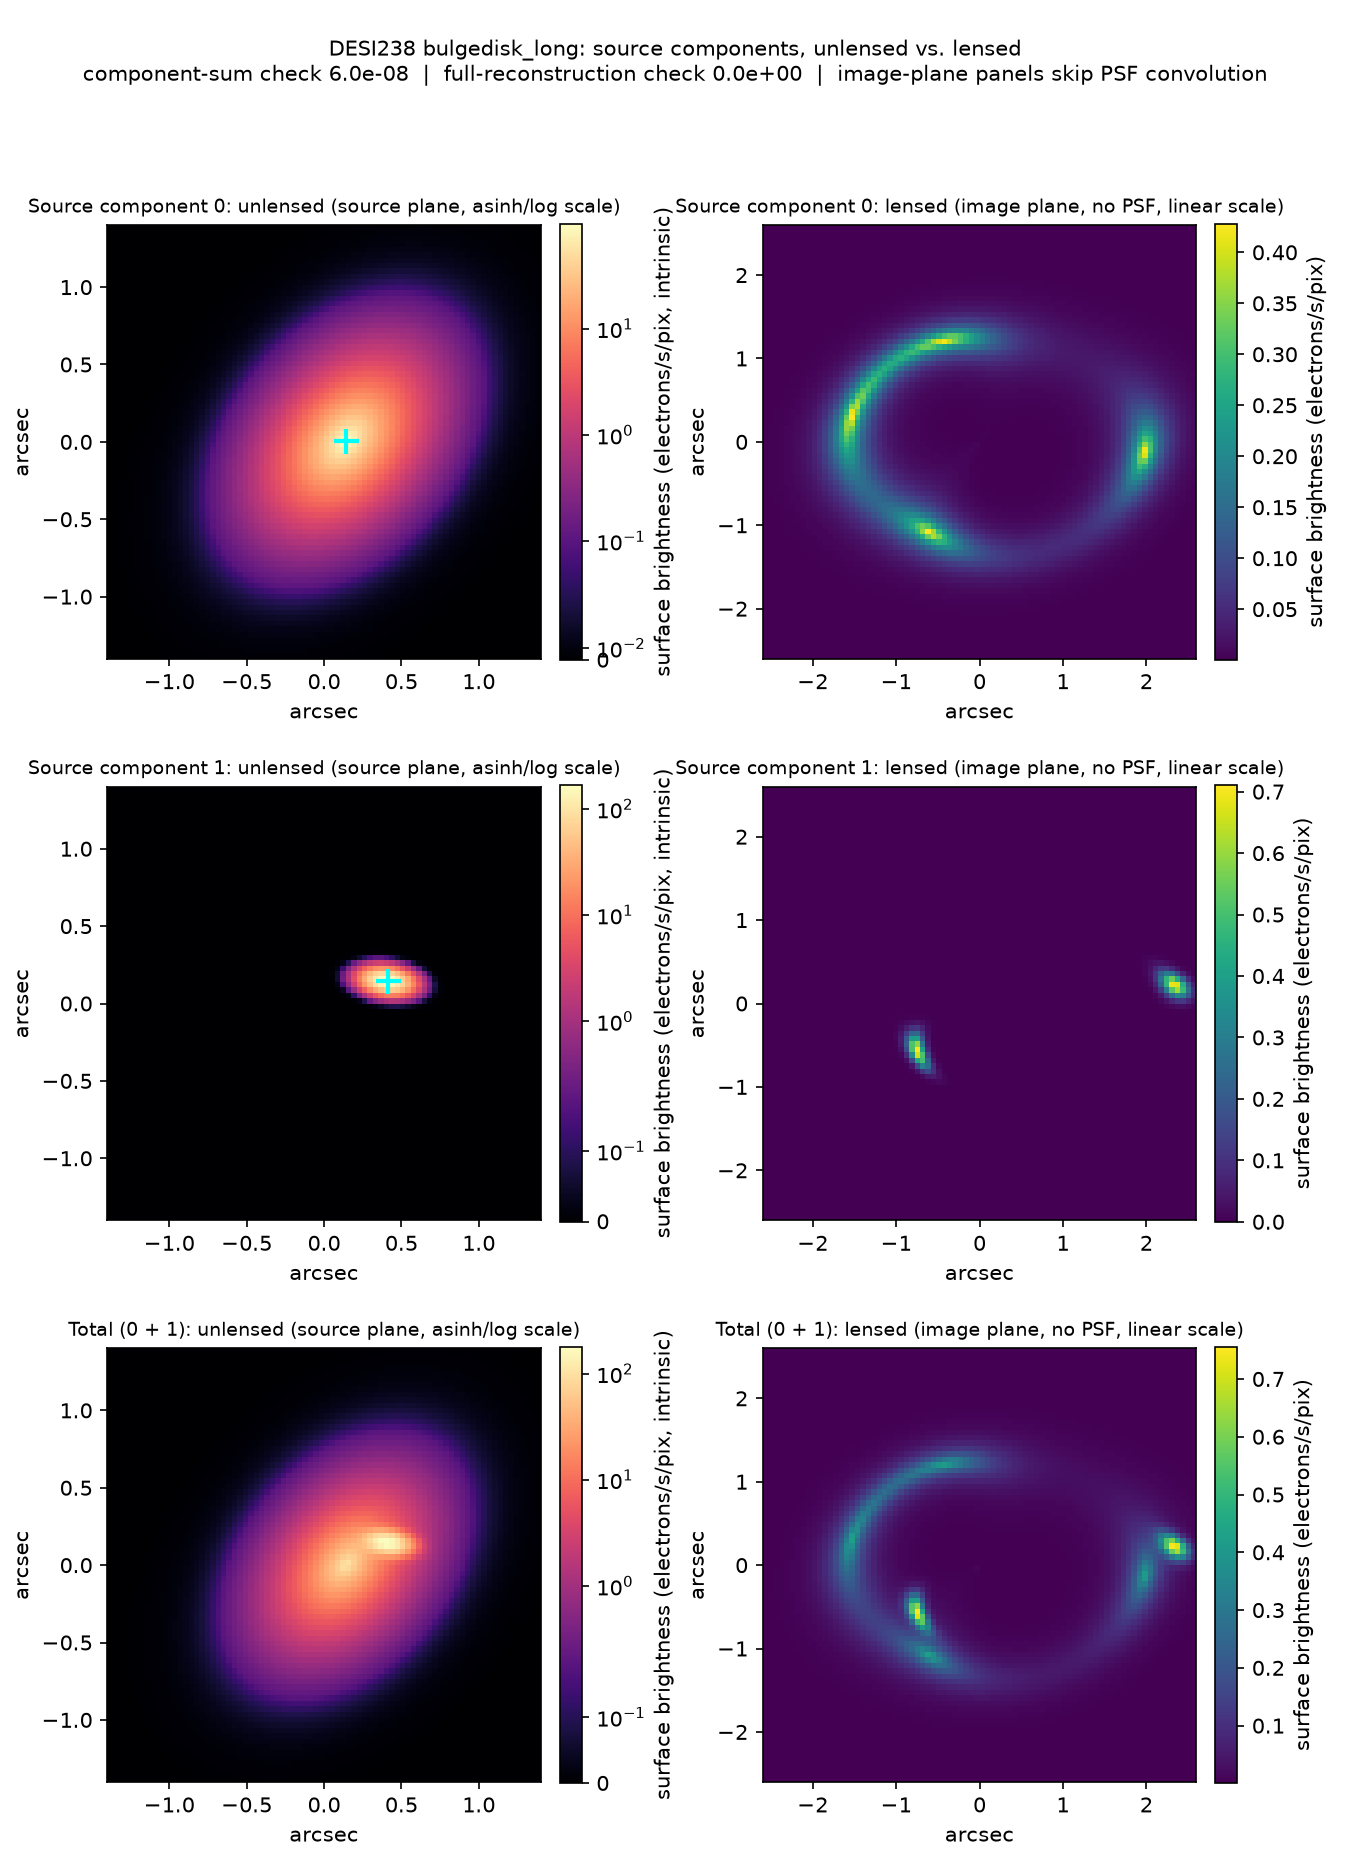
\includegraphics[width=0.7\textwidth]{source_components.png}
  \caption{The two source components, unlensed (left column) and lensed (right).
    Component 0 lenses into the full ring; component 1 produces two detached
    counter-images. The sum of the two lensed components reproduces the full model image
    to $6\times10^{-8}\,\mathrm{e^{-}\,s^{-1}}$, confirming the decomposition is exact
    and not an approximation.}
  \label{fig:source}
\end{figure}

The two components are an extended host and a compact knot. Their half-light radii differ
by only $3.2\times$ ($0.209\arcsec$ against $0.066\arcsec$); component~0 looks far larger
in Figure~\ref{fig:source} than that ratio suggests because the display is stretched and
because component~1, at $n = 0.52$, is sub-exponential and has no wings --- its surface
brightness falls sixteen orders of magnitude by $r = 0.5\arcsec$, so there is nothing to
render outside its core. Measured at fixed surface-brightness thresholds the ratio is
$3.2$, $4.0$, and $4.8\times$ at $\mathrm{SB} = 1.0$, $0.1$, and $0.01$.

The knot is $4.2\times$ brighter than the host in $I_{e}$ and offset from it by
$0.44\arcsec$. That offset is what makes the second component earn its place: the astroid
caustic in Figure~\ref{fig:overview} is only ${\sim}0.5\arcsec$ across, so the host, with
$R_{\mathrm{sersic}} = 0.209\arcsec$, is comparable in size to the caustic and smears into
a ring, while the knot straddles a fold and produces the detached images the data
requires. A single source component can make one behaviour or the other, not both.

\section{Model comparison}
\label{sec:comparison}

The bulge$+$disk deflector light was motivated by a coherent $1$--$3\%$ radial S-curve in
the core residual of the preceding fit --- over-bright at $r < 1$~pix, too faint at
$1.5$--$5.5$~pix, too bright again at $6.5$--$11.5$~pix. A single S\'ersic is a one-shape
family and cannot produce that pattern at any parameters. Table~\ref{tab:compare} gives
the comparison against the otherwise identical 29-parameter model, evaluated at each
run's point estimate over $N = 6400$ pixels.

\begin{table}[htbp]
  \centering
  \caption{Model comparison. $\Delta\log L = +911.9$ for seven added parameters;
    $\Delta\mathrm{AIC} = -1810$, $\Delta\mathrm{BIC} = -1762$. BIC charges
    $\ln 6400 \approx 8.8$ per parameter against a return of ${\sim}130$ per parameter,
    so the penalty is irrelevant at this margin.}
  \label{tab:compare}
  \begin{tabular}{lS[table-format=2]S[table-format=4.1]S[table-format=1.4]S[table-format=1.4]S[table-format=5.1]S[table-format=-6.1]}
    \toprule
    Model & {$k$} & {$\chi^{2}$} & {$\chi^{2}/N$} & {$\chi^{2}/(N-k)$} & {$\log L$} & {BIC} \\
    \midrule
    1 lens light (\texttt{twosource\_v2}) & 29 & 8170.5 & 1.2766 & 1.2824 & 18146.6 & -36039.0 \\
    2 lens light (\texttt{bulgedisk})     & 36 & 6340.6 & 0.9907 & 0.9963 & 19058.4 & -37801.4 \\
    \bottomrule
  \end{tabular}
\end{table}

Two qualifications. This is a maximum-likelihood comparison at point estimates, not a
Bayes factor; a marginal likelihood would penalise the 36-parameter model's larger prior
volume more heavily, though not by 1762. And because \texttt{ForwardProbModel}'s
$\sigma$ depends on the model image, the $-\sum \log \sigma$ normalisation is not constant
between the two models. We checked its size rather than assuming it away: it contributes
about $-3$ of the $+912$, so the comparison is carried by $\chi^{2}$.

Adding the second deflector component took the core $\chi^{2}$ ($r \le 8$~pix) from
$7.09$ to $2.97$ and flattened the S-curve into sign-alternating scatter within
$\pm0.75\sigma$. The central pixel improved from $-3.9\sigma$ to $-1.5\sigma$. Crucially,
it did not do this by eating arc flux --- the main risk, since a flexible light component
near the Einstein radius can absorb arc surface brightness and bias \thetaE. Aperture
ratios on the four clumps went $1.09 \to 1.03$ (SW arc), $0.99 \to 0.99$ (E blob),
$1.02 \to 1.02$ (W clump), and $0.91 \to 0.83$ (N arc), and \thetaE\ moved only
$1.484 \to 1.480\arcsec$.

\section{The noise scale}
\label{sec:noise}

$\chisqv = 0.989$ should not be read as evidence that the noise model is now correct.
$\sigma_{\mathrm{bkg}}$ is a single number drawn from six blank patches spanning
$0.0070$--$0.0092$, and \chisqv\ scales as $\sigma_{\mathrm{bkg}}^{-2}$:

\begin{table}[htbp]
  \centering
  \caption{Sensitivity to the background dispersion. A $\pm10\%$ error on
    $\sigma_{\mathrm{bkg}}$ is $\pm20\%$ on \chisqv --- larger than the distance from
    unity. The model comparison is untouched, because both models are evaluated under the
    same noise map and the scale factor largely cancels.}
  \label{tab:noise}
  \begin{tabular}{S[table-format=1.4]S[table-format=1.3]S[table-format=1.3]S[table-format=-4.0]}
    \toprule
    {$\sigma_{\mathrm{bkg}}$} & {$\chi^{2}/N$, 29 par} & {$\chi^{2}/N$, 36 par} & {$\Delta$BIC} \\
    \midrule
    0.0070 & 1.348 & 1.049 & -1848 \\
    0.0075 & 1.277 & 0.991 & -1762 \\
    0.0092 & 1.073 & 0.824 & -1526 \\
    \bottomrule
  \end{tabular}
\end{table}

Quote the improvement, not the absolute value. This makes building a per-pixel exposure
map from the drizzle product's \texttt{WHT} extension \emph{more} worth doing than before,
not less: at $\chisqv = 1.3$ the noise model was a second-order worry, and at $0.99$ it is
the leading systematic. The frame has $\mathtt{NCOMBINE} = 3$, so coverage genuinely
varies across it and a scalar $t_{\mathrm{exp}}$ understates the noise wherever fewer
exposures overlap.

\section{Convergence}
\label{sec:conv}

Two distinct failures had to be separated here, and confusing them cost a full round of
work.

The first was a diverged SVI stage. GIGA-Lens builds the HMC momentum distribution by
inverting the SVI covariance in float32. When that covariance is badly conditioned the
result is not an inverse: at the condition number of $8.8\times10^{11}$ reached in an
earlier run, $\max|C^{-1}C - I| = 55$ and the spectrum carried negative eigenvalues, so
every chain sampled against an effectively indefinite mass matrix and \emph{every}
$\hat{R}$ failed at once. The covariance was still positive definite, so a PD test does
not catch this --- conditioning is the discriminant. The cause was an SVI learning-rate
schedule that ramped upward, putting the largest steps last; replacing it with
warmup-then-decay took the conditioning to $3.8\times10^{7}$ for the run reported here.

The second was ordinary under-mixing, and the two are easy to confuse because both raise
every $\hat{R}$ at once. We separated them by brute force. The run reported here is
identical to its predecessor in every respect --- same seed, same priors, same MAP and SVI
settings, verified by an identical SVI starting loss --- except for chain length:

\begin{table}[htbp]
  \centering
  \caption{Effect of chain length at fixed model and fixed preconditioner. $\hat{R}$ fell
    toward unity rather than plateauing near 3, which is the outcome that says the
    geometry is samplable and the chains were simply too short. No reparametrisation is
    needed.}
  \label{tab:conv}
  \begin{tabular}{lcc}
    \toprule
     & \texttt{bulgedisk} & \texttt{bulgedisk\_long} \\
    \midrule
    draws $\times$ burn-in        & $750 \times 250$ & $3000 \times 1000$ \\
    worst $\hat{R}$               & 3.242            & \textbf{1.338} \\
    parameters with $\hat{R}>1.01$& 33/36            & \textbf{10/36} \\
    \chisqv                       & 0.991            & 0.989 \\
    SVI covariance condition      & $3.0\times10^{7}$& $3.8\times10^{7}$ \\
    \bottomrule
  \end{tabular}
\end{table}

What still fails is confined and interpretable: the two deflector components' shape
parameters, and \texttt{source1.n\_sersic}. The latter is the worst in the run
($\hat{R} = 1.338$, $\mathrm{ESS} = 201$) and is pinned at the $0.5$ lower bound of its
prior, sitting $0.4\%$ into its range. A parameter on a boundary cannot mix, so its
$\hat{R}$ is a symptom of the pinning and not independent evidence of anything. The floor
itself is deliberate: GIGA-Lens uses $b_{n} = 1.9992n - 0.3271$, which is $3\%$ wrong at
$n = 0.5$ and $13.6\%$ wrong at $n = 0.3$, so the fix is a different profile rather than a
lower bound. This is the third consecutive round in which an $n_{\mathrm{sersic}}$ has
pinned at $0.5$, and it is the clearest unresolved defect in the model.

\texttt{lens\_light1.n\_sersic} sits at $80\%$ of its $\mathrm{Uniform}(0.5, 2.5)$ prior
and has the worst non-boundary $\hat{R}$ at $1.096$. Widening it is a change to the
prior's \emph{support}, which silently rewrites the physical values of stored runs (the
checkpoints hold unconstrained samples), so it requires a prior-version bump rather than
an edit in place. It was deliberately left out of the long run so as not to confound the
one thing that run was measuring.

All eight mass parameters have $\hat{R} \le 1.002$. The non-convergence never touched the
lensing.

\section{Result and outstanding work}

\begin{equation}
  \thetaE = 1.480 \pm 0.003\arcsec, \qquad \hat{R} = 1.001, \quad \mathrm{ESS} = 94{,}186.
\end{equation}

This is the first error bar from a multi-component fit of this system that survives its
own diagnostic. It supersedes the $1.516 \pm 0.002\arcsec$ obtained from a
single-source, single-lens-light model of the same data. The two do not agree within their
quoted uncertainties, and they should not be expected to: the difference is a model
change, not a sampling one.

A model-to-model spread of this kind is a systematic uncertainty only when the models are
competitive --- when the data cannot decide between them, so both remain live and the
spread measures a genuine ambiguity. That is not the case here. Evaluated at the point
estimates over $N = 6400$ pixels, the round-1 model gives $\chi^2 \approx 11{,}757$ for
$k = 22$ against $6340.6$ for $k = 36$: $\Delta \log L \approx +2708$ for $14$ added
parameters, or $\Delta\mathrm{BIC} \approx -5294$ against a BIC penalty of only $123$.
\textbf{The single-component model is decisively rejected, so the $0.036\arcsec$ gap is
the size of a bias that has been removed, not an uncertainty that remains.} The quotable
uncertainty is the $\pm 0.003\arcsec$ above; inflating it to span a rejected model would
report a range the data has already excluded.

Two caveats survive. All $\Delta\log L$ and $\Delta\mathrm{BIC}$ values here are evaluated
at point estimates, so they are maximum-likelihood comparisons rather than Bayes factors;
a marginal likelihood would penalise the larger prior volume of the 36-parameter model
more heavily, though not by enough to close a gap of this size. And $\pm 0.003\arcsec$ is
the statistical error \emph{within the adopted model family}: it does not cover the noise
model, the single-scalar exposure time, or the EPL mass parametrisation, none of which
this comparison probes.

Four things remain open, in the order in which they gate a stronger result:

\begin{enumerate}
  \item \textbf{Whether the E blob is a counter-image.} This is the actual science
    question and it is still untested. A falsification run with \thetaE\ truncated below
    ${\sim}1.7\arcsec$ would settle it; earlier attempts used a prior whose $99$th
    percentile already admitted the four-image solution and so tested nothing. Deferring
    it was defensible while the source model was inadequate --- a failed A/B could be
    blamed on the model --- but at $\chisqv \approx 1$ that excuse is gone. Note that the
    E blob sits at $2.11\arcsec$, outside the tangential critical curve at $1.55\arcsec$,
    which bears directly on the interpretation.
  \item \textbf{The per-pixel exposure map from \texttt{WHT}}, for the reasons in
    \S\ref{sec:noise}.
  \item \textbf{The pinned $n_{\mathrm{sersic}} = 0.5$}, which needs a profile change, not
    a wider bound.
  \item \textbf{The core striping}, which the earlier colormap explanation does not
    obviously cover.
\end{enumerate}

\section*{Reproducing this}

{\small
\begin{verbatim}
export PYTHONPATH=gigalens/src:claude/pipeline NCCL_NVLS_ENABLE=0
CUDA_VISIBLE_DEVICES=0 python claude/pipeline/run_fit.py --lens DESI238 \
    --label bulgedisk_long --seed 0 --lens-light-n-max 10 \
    --n-source 2 --n-lens-light 2 --max-leapfrog 60 \
    --num-results 3000 --burnin 1000
python claude/pipeline/diagnose.py    claude/DESI238/runs/bulgedisk_long
python claude/pipeline/dump_params.py claude/DESI238/runs/bulgedisk_long
python claude/pipeline/plot_corner.py claude/DESI238/runs/bulgedisk_long
python claude/pipeline/plot_source.py claude/DESI238/runs/bulgedisk_long
python claude/pipeline/plot_overview.py claude/DESI238/runs/bulgedisk_long
\end{verbatim}
}

\noindent
The fit takes ${\sim}20$ minutes of HMC on one H100 and holds $62.7$ of $80$~GB; memory,
not compute, is what bounds a further increase in chain length. Full narrative notes are
in \texttt{RESULTS\_v3.md}, alongside the model code. The model comparison of
\S\ref{sec:comparison} came from a scratch script that is not checked in, but its numbers
are reproduced there.

\end{document}
